\documentclass[12pt]{article}
\usepackage{afterpage}
\usepackage{amsmath}
\usepackage{amsfonts}
\usepackage{amssymb}
\usepackage{amsbsy}
\usepackage{bm}
\usepackage{epsfig}
\usepackage{rotating}
\usepackage{setspace}
\usepackage{tabls}
\usepackage{hhline}
\usepackage{float}
% \usepackage{subfigure}
\usepackage{subcaption}
\usepackage{float}
\usepackage{xspace}
\usepackage{siunitx}
\DeclareSIUnit\particles{particles}
\sisetup{per-mode=fraction, inter-unit-product={}\cdot{}}
%\usepackage{subfigmat}
%\usepackage{citesort}
%\usepackage{cites}
%\usepackage{overcite}
%\usepackage[section]{placeins}

% uncomment for submission of manuscript to NSE
% \usepackage[nolists, nomarkers]{endfloat}
%
% use to include postscript figures
\usepackage{graphicx,color}
%
%\usepackage[light,firsttwo]{draftcopy}
%\draftcopySetGrey{0.90}

%\usepackage{dbl}

% -----------------------------------------------------------------------------
% define newcommands
% -----------------------------------------------------------------------------

%\setlength{\floatsep}{4pt plus 1pt minus 1pt}
%\setlength{\textfloatsep}{8pt plus 1pt minus 1pt}
%\setlength{\intextsep}{4pt plus 1pt minus 1pt}
%\setlength{\abovedisplayskip}{4pt plus 1pt minus 1pt}
%\setlength{\belowdisplayskip}{4pt plus 1pt minus 1pt}

% \makeatletter
% \renewcommand{\@thesubfigure}{\thefigure\thesubfigure\space}
% \makeatother
% =================================================================================================
% more new commands
% +++++++++++++++++++++++++++++++++++++++++++++++++++++++++++++++++++++++++++++++++++++++++++++++++
\setlength{\textwidth}{6.5in}
\setlength{\textheight}{8.in}
\setlength{\oddsidemargin}{0in}
%\setlength{\topmargin}{0.75in}
\setlength{\headsep}{12pt}
%\addtolength{\oddsidemargin}{-0.5in}
%\addtolength{\textwidth}{1.0in}
%\addtolength{\textheight}{1.0in}
\renewcommand{\thefootnote}{\fnsymbol{footnote}}
%
% -----------------------------------------------------------------------------
% define newcommands
% -----------------------------------------------------------------------------

%\setlength{\floatsep}{4pt plus 1pt minus 1pt}
%\setlength{\textfloatsep}{8pt plus 1pt minus 1pt}
%\setlength{\intextsep}{4pt plus 1pt minus 1pt}
%\setlength{\abovedisplayskip}{4pt plus 1pt minus 1pt}
%\setlength{\belowdisplayskip}{4pt plus 1pt minus 1pt}

% =================================================================================================
% more new commands
% +++++++++++++++++++++++++++++++++++++++++++++++++++++++++++++++++++++++++++++++++++++++++++++++++

% Ways of grouping things
%
\newcommand{\bracket}[1]{\left[ #1 \right]}
\newcommand{\bracet}[1]{\left\{ #1 \right\}}
\newcommand{\fn}[1]{\left( #1 \right)}
\newcommand{\ave}[1]{\left\langle #1 \right\rangle}
%
% Derivative forms
%
\newcommand{\dx}[1]{\,d#1}
\newcommand{\dxdy}[2]{\frac{\partial #1}{\partial #2}}
\newcommand{\dxdt}[1]{\frac{\partial #1}{\partial t}}
\newcommand{\dxdz}[1]{\frac{\partial #1}{\partial z}}
\newcommand{\dddx}[1]{\frac{d #1}{d x}}
\newcommand{\dfdt}[1]{\frac{\partial}{\partial t} \fn{#1}}
\newcommand{\dfdz}[1]{\frac{\partial}{\partial z} \fn{#1}}
\newcommand{\ddt}[1]{\frac{\partial}{\partial t} #1}
\newcommand{\ddz}[1]{\frac{\partial}{\partial z} #1}
\newcommand{\dd}[2]{\frac{\partial}{\partial #1} #2}
\newcommand{\ddx}[1]{\frac{\partial}{\partial x} #1}
\newcommand{\ddy}[1]{\frac{\partial}{\partial y} #1}
\newcommand{\ddxf}{\frac{d}{dx}}
%
% Vector forms 
%
%\renewcommand{\vec}[1]{\ensuremath{\stackrel{\rightarrow}{#1}}}
%\renewcommand{\div}{\ensuremath{\vec{\nabla} \cdot}}
%\newcommand{\grad}{\ensuremath{\vec{\nabla}}}
\renewcommand{\vec}[1]{\overrightarrow{#1}}
\renewcommand{\div}{\vec{\nabla}\! \cdot \!}
\newcommand{\grad}{\vec{\nabla}}
\newcommand{\oa}[1]{\fn{\frac{1}{3}\hat{\Omega}\!\cdot\!\overrightarrow{A_{#1}}}}

%
% Equation beginnings and endings
%
\newcommand{\bea}{\begin{eqnarray}}
\newcommand{\eea}{\end{eqnarray}}
\newcommand{\be}{\begin{equation}}
\newcommand{\ee}{\end{equation}}
\newcommand{\beas}{\begin{eqnarray*}}
\newcommand{\eeas}{\end{eqnarray*}}
\newcommand{\bdm}{\begin{displaymath}}
\newcommand{\edm}{\end{displaymath}}


%
% Equation punctuation
%
\newcommand{\pec}{\; ,}
\newcommand{\pep}{\; .}
%
% Equation labels and references, figure references, table references
%
\newcommand{\LEQ}[1]{\label{eq:#1}}
\newcommand{\EQ}[1]{Eq.~(\ref{eq:#1})}
\newcommand{\EQS}[1]{Eqs.~(\ref{eq:#1})}
\newcommand{\REQ}[1]{\ref{eq:#1}}
\newcommand{\LFI}[1]{\label{fi:#1}}
\newcommand{\FI}[1]{Fig.~\ref{fi:#1}}
\newcommand{\RFI}[1]{\ref{fi:#1}}
\newcommand{\LTA}[1]{\label{ta:#1}}
\newcommand{\TA}[1]{Table~\ref{ta:#1}}
\newcommand{\RTA}[1]{\ref{ta:#1}}

%
% List beginnings and endings
%
\newcommand{\bl}{\bss\begin{itemize}}
\newcommand{\el}{\vspace{-.5\baselineskip}\end{itemize}\ess}
\newcommand{\ben}{\bss\begin{enumerate}}
\newcommand{\een}{\vspace{-.5\baselineskip}\end{enumerate}\ess}
%
% Figure and table beginnings and endings
%
\newcommand{\bfg}{\begin{figure}}
\newcommand{\efg}{\end{figure}}
\newcommand{\bt}{\begin{table}}
\newcommand{\et}{\end{table}}
%
% Tabular and center beginnings and endings
%
\newcommand{\bc}{\begin{center}}
\newcommand{\ec}{\end{center}}
\newcommand{\btb}{\begin{center}\begin{tabular}}
\newcommand{\etb}{\end{tabular}\end{center}}
%
% Single space command
%
%\newcommand{\bss}{\begin{singlespace}}
%\newcommand{\ess}{\end{singlespace}}
\newcommand{\bss}{\singlespacing}
\newcommand{\ess}{\doublespacing}
%
%---New environment "arbspace". (modeled after singlespace environment
%                                in Doublespace.sty)
%   The baselinestretch only takes effect at a size change, so do one.
%
\def\arbspace#1{\def\baselinestretch{#1}\@normalsize}
\def\endarbspace{}
\newcommand{\bas}{\begin{arbspace}}
\newcommand{\eas}{\end{arbspace}}
%
% An explanation for a function
%
\newcommand{\explain}[1]{\mbox{\hspace{2em} #1}}
%
% Quick commands for symbols
%
\newcommand{\half}{\frac{1}{2}}
\newcommand{\halff}{1/2}
\newcommand{\third}{\frac{1}{3}}
\newcommand{\twothird}{\frac{2}{3}}
\newcommand{\mdot}{\dot{m}}
\newcommand{\ten}[1]{\times 10^{#1}\,}
\newcommand{\cL}{{\cal L}}
\newcommand{\cD}{{\cal D}}
\newcommand{\cF}{{\cal F}}
\newcommand{\cE}{{\cal E}}
\renewcommand{\Re}{\mbox{Re}}
\newcommand{\Ma}{\mbox{Ma}}
% 
% Inclusion of Graphics Data
%
%\input{psfig}
%\psfiginit
%
% More Quick Commands
%
\newcommand{\bi}{\begin{itemize}}
\newcommand{\ei}{\end{itemize}}
\newcommand{\dxi}{\Delta x_i}
\newcommand{\dyj}{\Delta y_j}
\newcommand{\ts}[1]{\textstyle #1}
% Mark URL's
\newcommand{\URL}[1]{{\textcolor{blue}{#1}}}



% Alter some LaTeX defaults for better treatment of figures:
    % See p.105 of "TeX Unbound" for suggested values.
    % See pp. 199-200 of Lamport's "LaTeX" book for details.
    %   General parameters, for ALL pages:
    \renewcommand{\topfraction}{0.9}	% max fraction of floats at top
    \renewcommand{\bottomfraction}{0.8}	% max fraction of floats at bottom
    %   Parameters for TEXT pages (not float pages):
    \setcounter{topnumber}{2}
    \setcounter{bottomnumber}{2}
    \setcounter{totalnumber}{2}     % 2 may work better
    \setcounter{dbltopnumber}{2}    % for 2-column pages
    \renewcommand{\dbltopfraction}{0.9}	% fit big float above 2-col. text
    \renewcommand{\textfraction}{0.07}	% allow minimal text w. figs
    %   Parameters for FLOAT pages (not text pages):
    \renewcommand{\floatpagefraction}{0.7}	% require fuller float pages
	% N.B.: floatpagefraction MUST be less than topfraction !!
    \renewcommand{\dblfloatpagefraction}{0.7}	% require fuller float pages

	% remember to use [htp] or [htpb] for placement 

\newcommand{\SN}{S$_N$\xspace}
\renewcommand{\vec}[1]{\bm{#1}} %vector is bold italic
\newcommand{\vd}{\bm{\cdot}} % slightly bold vector dot
\newcommand{\ud}{\mathop{}\!\mathrm{d}} % upright derivative symbol
\newcommand{\pderiv}[2]{\frac{\partial #1}{\partial #2}}
\newcommand{\dderiv}[2]{\frac{d #1}{d #2}}
\newcommand{\edd}{\langle \mu^2 \rangle} 	
	
% =================================================================================================
\date{}

\begin{document}

%\bibliographystyle{nse}
%\bibnum{p}

\thispagestyle{empty}
\bc
{\Large \bf Variable Eddington Factor Method for the \SN Equations with Lumped Discontinuous Galerkin Spatial Discretization 
Coupled to a Drift-Diffusion Acceleration Equation with Mixed Finite-Element Discretization}\\
\vspace{0.5in}
{\large {\bf Samuel S. Olivier, Jim E. Morel}\\
$ $\\
Department of Nuclear Engineering\\
Texas A\&M University\\
College Station, TX 77843}\\
\ec
$ $\\
\bc
{\large \bf Abstract}\\
\ec
\noindent
\emph{
%!TEX root = ./jctt.tex
We present the Variable Eddington Factor (VEF) method, a nonlinear Discrete Ordinates Source Iteration scheme that relaxes the consistency requirement of the transport and acceleration steps' spatial discretization. The method was applied to the 1-D, one-group neutron transport equation with Lumped Linear Discontinuous Galerkin (LLDG) transport and the constant-linear Mixed Finite Element Method (MFEM) drift diffusion acceleration. Methods for increased consistency between the transport and acceleration steps are also presented. The VEF method exhibited second-order convergence as expected from the orders of accuracy of LLDG and MFEM in isolation, accelerated source iterations as well as consistently differenced S$_2$SA, and survived the thick diffusion limit. In addition, the difference between the transport and acceleration steps' solution was shown to converge as the mesh was refined. 
}\\
$ $\\
\noindent
{\bf Keywords}\\
\noindent Variable Eddington Factor, Source Iteration Acceleration, Lumped Linear Discontinuous Galerkin, Mixed Finite Element Method  \\
$ $\\
\noindent {\bf Running Head}\\
\noindent Variable Eddington Factor Method \\
$ $\\
\noindent{\bf Corresponding Author}\\
\noindent Samuel S. Olivier, email: \emph{smsolivier@gmail.com}. 
$ $\\
\newpage
\ess

\setcounter{page}{1} % reset page count to ignore title page 
\section{Introduction}
%!TEX root = ./jctt.tex
The Variable Eddington Factor (VEF) method, also known as Quasi-Diffusion (QD), was one of the first nonlinear methods 
for accelerating source iterations in \SN calculations \cite{AL}.  It is comparable in effectiveness to both linear 
and nonlinear forms of Diffusion-Synthetic Acceleration (DSA), but it offers much more flexibility than the DSA.   
Stability can only be guaranteed with DSA if the diffusion equation is differenced in a manner consistent with that 
of the \SN equations \cite{A}. Modern \SN codes often use advanced discretization schemes such as discontinuous 
Galerkin (DG) since classic discretization schemes such as step and diamond are not suitable for radiative transfer 
calculations in the High Energy Density Laboratory Physics (HEDLP) regime or coupled electron-photon calculations.  
Diffusion discretizations consistent 
with DG \SN discretizations cannot actually be expressed in diffusion form, but rather must be expressed in 
first-order or P$_1$ form, and are much more difficult to solve than standard diffusion discretizations \cite{WWM}.  Considerable 
effort has gone into the development of ``partially consistent'' diffusion discretizations that yield a stable DSA 
algorithm with some degree of degraded effectiveness, but such discretizations are also generally difficult to develop \cite{ML,AM,WR}. 
A great advantage of the VEF method is that the drift-diffusion equation that accelerates the \SN source iterations can be 
discretized in any valid manner without concern for consistency with the \SN discretization.  When the VEF 
drift-diffusion equation is discretized in a way that is ``non-consistent,'' the \SN and VEF drift-diffusion solutions 
for the scalar flux do not necessarily become identical when the iterative process converges.  However, they do become 
identical in the limit as the spatial mesh is refined, and the difference between the two solutions is proportional to 
the spatial truncation errors associated with the \SN and drift-diffusion discretizations.  In general the order accuracy 
of the \SN and VEF drift-diffusion solutions will be the lowest order accuracy of their respective independent 
discretizations.  Although the \SN solution obtained with such a ``non-consistent'' VEF method is not conservative, 
the VEF drift-diffusion solution is in fact conservative.  This is particularly useful in multiphysics calculations 
where the low-order VEF equation can be coupled to the other physics components rather than the high-order \SN 
equations.  Another advantage of the non-consistent approach is that even if the \SN spatial discretization 
scheme does not preserve the thick diffusion limit \cite{LMM}, that limit will generally be preserved using the VEF method. 
 
The purpose of this paper is to investigate the application of the VEF method with the 1-D \SN equations 
discretized with the lumped linear-discontinuous method (LLDG) and the drift-diffusion equation discretized using the 
constant-linear mixed finite-element method (MFEM).  To our knowledge, this combination has not been previously 
investigated.  Our motivation for this investigation is that MFEM methods are now being used for high-order hydrodynamics 
calculations \cite{blast}.  A radiation transport method compatible with MFEM 
methods is clearly desirable for developing a MFEM radiation-hydrodynamics code.  Such a code would combine thermal 
radiation transport with hydrodynamics.  However, MFEM methods are inappropriate for the standard first-order form of the 
transport equation.    
Thus the use of the VEF method with a DG \SN discretization and a MFEM drift-diffusion discretization suggests itself.
Here we define a VEF method that should exhibit second-order accuracy since both the transport and drift-diffusion 
discretizations are second-order accurate in isolation.  In addition, our VEF method should preserve the thick diffusion 
limit, which is essential for radiative transfer calculations in the HEDLP regime. We use the lumped 
rather than the standard Linear Discontinuous Galerkin discretization because lumping yields a much more robust scheme, and robustness is essential 
for radiative transfer calculations in the HEDLP regime.   Because this is an initial study, we simplify the investigation 
by considering only the one-group neutron transport equation rather than the full radiative transfer equations, which include a 
material temperature equation as well as the radiation transport equation.  The vast majority of relevant properties of  
a VEF method for radiative transfer can be tested with an analogous method for one-group neutron transport.  Furthermore, 
a high-order DG-MFEM VEF method could be of interest for neutronics in addition to radiative transfer calculations. 
A full investigation for radiative transfer calculations will be carried out in a future study. 

The remainder of this paper is organized as follows.  First, we describe the VEF method analytically. Then we describe 
our discretized \SN equations, followed by a description of the discretized VEF drift-diffusion equation.  We next give 
computational results.  More specifically, we describe 
two ways to represent the \SN variable Eddington factor in the MHEM drift-diffusion equation and several ways to 
construct the \SN scattering source from the drift-diffusion solution for the scalar flux. Each of these options 
yields a different VEF method.  The accuracy of these methods is then compared to that of the standard LLDG 
\SN solution for several test problems, and the iterative convergence rate of these methods is compared to that of the 
LLDG \SN equations with fully-consistent S$_2$SA acceleration. Finally, we give conclusions and 
recommendations for future work.

% \begin{thebibliography}{99}
% \bibitem{AL} M.L.  Adams  and  E.W.  Larsen,  ``Fast  Iterative  Methods  for  Discrete-Ordinates  Particle  Transport 
% Calculations,''  {\it Progress in Nuclear Energy}, {\bf 40(1)}, 3--159 (2002).
% \bibitem{A} R.E. Alcouffe, ``Diffusion Synthetic Acceleration Methods for the Diamond-Differenced Discrete-Ordinates 
% Equations,'' {\it Nuclear Science and Engineering}, {\bf 64}, 344--355 (1977).
% \bibitem{WWM} J.S. Warsa, T.A. Wareing, and J.E. Morel, ``Fully-Consistent Diffusion-Synthetic Acceleration 
% of Linear Discontinuous $S_n$ Transport Discretizations on Unstructured Tetrahedral Meshes,'' 
% {\em Nuclear Science and Engineering}, {\bf 141}, 235-251 (2002).
% \bibitem{ML} J.E. Morel and E.W. Larsen, ``A Multiple Balance Approach for Differencing the $S_n$ Equations,'' 
% {\em Nuclear Science and Engineering}, {\bf 105}, 1-15 (1990).
% \bibitem{AM} Marvin L. Adams and William R. Martin, ``Diffusion Synthetic Acceleration of Discontinuous Finite Element 
% Transport Iterations,'' {\it Nuclear Science and Engineering}, {\bf 111}, 145--167 (1992).
% \bibitem{WR} Yaqi Wang, Jean C. Ragusa, ``Diffusion Synthetic Acceleration for High-Order Discontinuous Finite Element \SN 
% Transport Schemes and Application to Locally Refined Unstructured Meshes,'' {\it Nuclear Science and Engineering}, {\bf 166(2)}, 
% 145--166 (2010).
% \bibitem{LMM} Edward W. Larsen, J.E. Morel, Warren F. Miller, Jr., ``Asymptotic Solutions of Numerical Transport 
% Problems in Optically Thick, Diffusive Regimes,'' {\em Journal of Computational Physics}, {\bf 69},  283-324 (1987).
% \bibitem{blast} V. Dobrev, Tz. Kolev and R. Rieben, ``High-Order Curvilinear Finite Element Methods for Lagrangian Hydrodynamics,'' 
% {\it SIAM Journal on Scientific Computing, {\bf 34), B606�-B641 (2012).
% \end{thebibliography}

%!TEX root = ./jctt.tex

\newcommand{\rell}{^\ell} % raise to ellth power 
\newcommand{\relll}{^{\ell+1}} % raise to ell + 1 th power 
\newcommand{\rellh}{^{\ell+1/2}} % raise to ell + 1/2 power

\newcommand{\paren}[1]{\left(#1\right)} 

\section{The VEF Method}
\subsection{The Algorithm}
Here, we describe the VEF method for a planar geometry, fixed-source problem:
	\begin{equation} 
		\mu \pderiv{\psi}{x} \paren{x, \mu} + \sigma_t(x) \psi(x,\mu) = 
			\frac{\sigma_s(x)}{2} \int_{-1}^1 \psi(x,\mu') \ud \mu' + \frac{Q(x)}{2} \,,
	\end{equation}
where $\mu = \cos\theta$ is the cosine of the angle of flight $\theta$ relative to the $x$--axis, $\sigma_t(x)$ and $\sigma_s(x)$ the total and scattering macroscopic cross sections, $Q(x)$ the isotropic fixed-source and $\psi(x, \mu)$ the angular flux. Applying the Discrete Ordinates (\SN) angular discretization yields the following set of $N$ coupled, ordinary differential equations: 
	\begin{equation} \label{eq:sn}
		\mu_n \dderiv{\psi_n}{x}(x) + \sigma_t(x) \psi_n(x) = 
		\frac{\sigma_s(x)}{2} \phi(x) + \frac{Q(x)}{2} \,, 1 \leq n \leq N \,,
	\end{equation}
where $\psi_n(x) = \psi(x, \mu_n)$ is the angular flux in direction $\mu_n$. The $\mu_n$ are stipulated by an $N$-point Gauss quadrature rule such that the scalar flux, $\phi(x)$, can be numerically integrated with: 
	\begin{equation} \label{eq:phiquad}
		\phi(x) = \sum_{n=1}^N w_n \psi_n(x) \,
	\end{equation}
where the $w_n$ are the quadrature weights corresponding to the $\mu_n$. 

The VEF method decouples Eq. \ref{eq:sn} by lagging the scattering term: 
	\begin{equation} \label{eq:si}
		\mu_n \dderiv{\psi_n\rellh}{x}(x) + \sigma_t(x) \psi_n\rellh(x) = 
		\frac{\sigma_s(x)}{2} \phi^\ell(x) + \frac{Q(x)}{2} \,, 1 \leq n \leq N \,,
	\end{equation}
where the superscripts indicate the iteration index. In Source Iteration (SI), the update 
	\begin{equation} \label{eq:siupdate}
		\phi(x)\relll = \phi(x)\rellh
	\end{equation}
is used. However, this is slow to converge in optically thick and highly scattering systems. Instead, the VEF method solves the VEF drift diffusion equations found by taking the first two moments of Eq. \ref{eq:sn}: 
	\begin{subequations} 
	\begin{equation} \label{eq:zero}
		\dderiv{}{x} J\relll(x) + \sigma_a(x) \phi\relll(x) = Q(x) \,,
	\end{equation} 
	\begin{equation} \label{eq:first}
		\frac{\ud}{\ud x} \edd\rellh(x) \phi\relll(x) + \sigma_t(x) J\relll(x) = 0 \,,
	\end{equation}
	\end{subequations}
where $J\relll(x)$ is the current and 
	\begin{equation} \label{eq:eddington} 
		\edd\rellh(x) = \frac{\int_{-1}^1 \mu^2 \psi\rellh(x, \mu) \ud \mu}{\int_{-1}^1 \psi\rellh(x, \mu) \ud \mu}
		\xrightarrow{\text{\SN}} \frac{
			\sum_{n=1}^N \mu_n^2 \psi_n\rellh(x) w_n
		}{
			\sum_{n=1}^N \psi_n\rellh(x) w_n 
		}
	\end{equation}
the Eddington factor. The scattering term in Eq. \ref{eq:si} is then updated with the VEF drift diffusion scalar flux found by solving Eqs. \ref{eq:zero} and \ref{eq:first}. This process of solving Eq. \ref{eq:si} for the $\psi_n(x)$, computing the Eddington factor, solving the VEF drift diffusion equation for the scalar flux, and updating the scattering term with the VEF drift diffusion scalar flux is repeated convergence. 

Acceleration occurs because the angular shape of the angular flux, and thus the Eddington factor, converges much faster than the scalar flux. In addition, the VEF equations model the contributions of all scattering events at once, reducing the dependence on source iterations to introduce scattering information. 
% The solution from the VEF equations is then an approximation for the full flux and not the $\ell - 1$ collided flux as it was without acceleration. 

In addition to acceleration, this scheme allows the \SN equations and drift diffusion equations to be solved with arbitrarily different spatial discretization methods. The following sections  present the application of the Lumped Linear Discontinuous Galerkin (LLDG) spatial discretization to the \SN equations and the Mixed Finite Element Method (MFEM) to the VEF drift diffusion equations. 

\subsection{Lumped Linear Discontinuous Galerkin \SN}
\begin{figure}
	\centering
	\input{figs/lldggrid.pdf_tex}
	\caption{The distribution of unknowns in an LLDG cell. The superscript $+$ and $-$ indicate the angular fluxes for $\mu_n>0$ and $\mu_n<0$, respectively. } 
\end{figure}
The LLDG discretization of Eq. \ref{eq:si} is: 
	\begin{subequations} 
	\begin{equation} \label{eq:lldg_l}
		\mu_n \left(\psi_{n,i}\rellh - \psi_{n, i-1/2}\rellh\right) 
		+ \frac{\sigma_{t,i} h_i}{2} \psi_{n,i,L}\rellh
		= \frac{\sigma_{s,i} h_i}{4} \phi_{i,L}\rell + \frac{h_i}{4} Q_{i,L} \,, 
		% 1 \leq n \leq N \,, 
		% 1 \leq i \leq I\,, 
	\end{equation}
	\begin{equation} \label{eq:lldg_r}
		\mu_n \left(\psi_{n,i+1/2}\rellh - \psi_{n,i}\rellh\right) 
		+ \frac{\sigma_{t,i} h_i}{2} \psi_{n,i,R}\rellh
		= \frac{\sigma_{s,i} h_i}{4} \phi_{i,R}\rell + \frac{h_i}{4} Q_{i,R} \,, 
		% 1 \leq n \leq N \,, 
		% 1 \leq i \leq I\,,
	\end{equation}
	\end{subequations}
where $h_i$, $\sigma_{t,i}$, and $\sigma_{s,i}$ are the cell width, total cross section, and scattering cross section in cell $i$. The $i,L$ and $i,R$ subscripts indicate the the subscripted value is the left or right discontinuous edge value. The cell centered angular flux is the average of the left and right discontinuous edge fluxes:
	\begin{equation} \label{eq:lldg_i}
		\psi_{n,i}\rellh = \half\left(\psi_{n,i,L}\rellh + \psi_{n,i,R}\rellh\right) \,.
	\end{equation}
The cell edged angular fluxes are defined through upwinding: 
	\begin{subequations}
	\begin{equation} \label{eq:downwind}
		\psi_{n,i-1/2}\rellh = \begin{cases}
			\psi_{n,i-1,R}\rellh \,, & \mu_n > 0 \\ 
			\psi_{n,i,L}\rellh \,, & \mu_n < 0 
		\end{cases} \,,
	\end{equation}
	\begin{equation} \label{eq:upwind}
		\psi_{n,i+1/2}\rellh = \begin{cases}
			\psi_{n,i,R}\rellh \,, & \mu_n > 0 \\
			\psi_{n,i+1,L}\rellh \,, & \mu_n < 0 
		\end{cases} \,.
	\end{equation}
	\end{subequations}
Equations \ref{eq:lldg_l}, \ref{eq:lldg_r}, \ref{eq:lldg_i}, \ref{eq:downwind}, and \ref{eq:upwind} can be combined and rewritten as 
	\begin{equation} \label{eq:sweepLR}
		\left[\begin{matrix}
			\mu_n + \sigma_{t,i} h_i & \mu_n  \\ 
			-\mu_n & \sigma_{t,i} + \mu_n \\ 
		\end{matrix}\right]
		\left[\begin{matrix}
			\psi_{n,i,L}\rellh \\ \psi_{n,i,R}\rellh
		\end{matrix}\right]
		= \left[\begin{matrix}
			\frac{\sigma_{s,i}h_i}{2} \phi_{i,L}\rell + \frac{h_i}{2} Q_{i,L} + 2\mu_n \psi_{n,i-1,R}\rellh \\
			\frac{\sigma_{s,i}h_i}{2} \phi_{i,R}\rell + \frac{h_i}{2} Q_{i,R} 
		\end{matrix}\right] \,, 
	\end{equation}
for sweeping from left to right ($\mu_n > 0$) and 
	\begin{equation} \label{eq:sweepRL}
		\left[\begin{matrix} 
			-\mu_n + \sigma_{t,i}h_i & \mu_n \\ 
			-\mu_n & -\mu_n + \sigma_{t,i}h_i \\ 
		\end{matrix} \right]
		\left[\begin{matrix}
			\psi_{n,i,L}\rellh \\ \psi_{n,i,R}\rellh
		\end{matrix} \right]
		= \left[\begin{matrix}
			\frac{\sigma_{s,i}h_i}{2} \phi_{i,L}\rell + \frac{h_i}{2} Q_{i,L} \\ 
			\frac{\sigma_{s,i}h_i}{2} \phi_{i,R}\rell + \frac{h_i}{2} Q_{i,R} - 2\mu_n \psi_{n,i+1,L}\rellh
		\end{matrix} \right]
		\,, 
	\end{equation}
for sweeping from right to left ($\mu_n < 0$). The right hand sides of Eqs. \ref{eq:sweepLR} and \ref{eq:sweepRL} are known as the scalar flux from the previous iteration, the fixed source, and the angular flux entering from the previous cell are all known. By supplying the flux entering the left side of the first cell, the positive-angled solution can be propagated from left to right by solving Eq. \ref{eq:sweepLR}. Similarly, supplying the incident flux on the right boundary allows the negative-angled solution to be propagated from right to left with Eq. \ref{eq:sweepRL}. 

\subsection{Mixed Finite Element Method VEF Drift Diffusion}
\begin{figure}
	\centering
	% \def\svgwidth{\textwidth}
	\input{figs/mfemgrid.pdf_tex} 
	\caption{The distribution of unknowns in cell $i$ for MFEM. }
\end{figure}
Applying the MFEM to Eqs. \ref{eq:zero} and \ref{eq:first} and enforcing continuity of current yields: 
	\begin{subequations} \label{eq:mfem}
	\begin{equation}
		-\frac{6}{\sigma_{t,i}h_i} \edd_{i-1/2} \phi_{i-1/2}
		+ \left(\frac{12}{\sigma_{t,i}h_i} \edd_i + \sigma_{a,i} h_i\right) \phi_i 
		- \frac{6}{\sigma_{t,i} h_i} \edd_{i+1/2} \phi_{i+1/2} 
		= Q_i h_i \,,
	\end{equation}
	\begin{multline}
		-\frac{2}{\sigma_{t,i} h_i} \edd_{i-1/2}\phi_{i-1/2} + 
		\frac{6}{\sigma_{t,i} h_i} \edd_i \phi_i 
		- 4\left(\frac{1}{\sigma_{t,i} h_i} + \frac{1}{\sigma_{t,i+1} h_{i+1}}\right) 
			\edd_{i+1/2} \phi_{i+1/2}
		\\ + \frac{6}{\sigma_{t,i+1} h_{i+1}} \edd_{i+1} \phi_{i+1} 
		- \frac{2}{\sigma_{t,i+1} h_{i+1}} \edd_{i+3/2} \phi_{i+3/2} 
		= 0 \,,
	\end{multline}
	\end{subequations}
where the Eddington factor is evaluated at iteration $\ell+1/2$ and the scalar flux at $\ell+1$. 
Here, the Eddington factor has been assumed to be constant in each cell with discontinuous jumps at the edges. 
The simplest method of converting the Eddington factor from LLDG to MFEM is to compute the Eddington factor using the cell centered and cell edged angular fluxes using Eqs. \ref{eq:lldg_i}, \ref{eq:downwind}, and \ref{eq:upwind}. A more consistent way to transfer the Eddington factor is to represent the LLDG angular flux as a linear function using the MFEM basis functions: 
	\begin{equation} \label{eq:eddquad}
		\edd_i(x) = \frac{
			\sum_{n=1}^N \mu_n^2 \left[\psi_{n,i,L}B_{i,L}(x) + \psi_{n,i,R} B_{i,R}(x)\right]
		}
		{
			B_{i,L}(x) \sum_{n=1}^N w_n \psi_{n,i,L} + B_{i,R}(x) \sum_{n=1}^N w_n \psi_{n,i,R} 
		} \,,
	\end{equation}
where 
	\begin{equation}
		B_{i,L}(x) = \begin{cases}
			\frac{x_{i+1/2} - x}{h_i} \,, & x \in [x_{i-1/2}, x_{i+1/2}] \\ 
			0 \,, & \text{otherwise}
		\end{cases}
	\end{equation}
and 
	\begin{equation}
		B_{i,R}(x) = \begin{cases}
			\frac{x - x_{i-1/2}}{h_i} \,, & x \in [x_{i-1/2}, x_{i+1/2}] \\ 
			0 \,, & \text{otherwise}
		\end{cases} \,.
	\end{equation}
When MFEM is applied, the integral over cell $i$ of the rational polynomial given in Eq. \ref{eq:eddquad} is approximated with 2 point Gauss quadrature. The cell centered Eddington factors used in Eq. \ref{eq:mfem} are then: 
	\begin{equation} 
		\edd_i = \half \left[ \edd_i(x_{i,L}) + \edd_i(x_{i,R}) \right] \,,
	\end{equation}
where 
	\begin{equation}
		x_{i,L/R} = \frac{x_{i+1/2} - x_{i-1/2}}{2} \mp \frac{x_{i+1/2} + x_{i-1/2}}{2\sqrt{3}}
	\end{equation}
are the quadrature points in cell $i$. 

Transport consistent boundary conditions are applied through a modified Marshak boundary condition: 
	\begin{equation} 
		J(x) = B(x) \phi(x) \,,
	\end{equation} 
where 
	\begin{equation} 
		B(x) = \frac{\int_{-1}^1 |\mu| \psi(x, \mu) \ud \mu}
		{\int_{-1}^1 \psi(x, \mu) \ud \mu} \,. 
	\end{equation}

Once the MFEM scalar flux has been found, the LLDG scattering term must be reconstructed. Two methods have been tested: no reconstruction and van Leer limited cell centered slope reconstruction. The no reconstruction method sets the LLDG discontinuous left and right scalar flux to the MFEM edge scalar flux: 
	\begin{equation} 
		\phi_{i,L/R} = \phi_{i\mp1/2} \,,
	\end{equation} 
where the left hand side is the reconstructed LLDG flux used in the scattering term of Eq. \ref{eq:si} and the right hand side the MFEM drift diffusion flux. The van Leer cell centered reconstruction is: 
	\begin{equation} 
		\phi_{i,L/R} = \phi_i \mp \frac{1}{4} \xi_\text{van Leer} \left[\left(\phi_{i+1} - \phi_i\right) + \left(\phi_i - \phi_{i-1}\right) \right] \,,
	\end{equation}
where $\xi_\text{van Leer}$ the slope limiter given in \cite{vanLeer}. 
%!TEX root = ./jctt.tex

\subsection{Mixed Finite Element Method VEF Drift Diffusion}
\begin{figure}
	\centering
	% \def\svgwidth{\textwidth}
	\input{figs/mfemgrid.pdf_tex} 
	\caption{The distribution of unknowns in cell $i$ for MFEM. }
	\label{fig:mfem_grid}
\end{figure}
The unknowns in an MFEM cell are depicted in Fig. \ref{fig:mfem_grid}. The scalar flux is constant within the cell with discontinuous jumps at the cell edges and the current is a linear function defined by: 
	\begin{equation} \label{eq:MFEM_current}
		J_i(x) = J_{i,L} B_{i,L}(x) + J_{i,R} B_{R,i}(x) \,, 
	\end{equation} 
where $J_{i,L/R}$ are the currents at the left and right edges of the cell and 
	\begin{subequations}
		\begin{equation}
			B_{i,L}(x) = \begin{cases}
				\frac{x_{i+1/2} - x}{h_i} \,, & x \in [x_{i-1/2}, x_{i+1/2}] \\ 
				0 \,, & \text{otherwise}
			\end{cases} \,,
		\end{equation}
		\begin{equation}
			B_{i,R}(x) = \begin{cases}
				\frac{x - x_{i-1/2}}{h_i} \,, & x \in [x_{i-1/2}, x_{i+1/2}] \\ 
				0 \,, & \text{otherwise}
			\end{cases} \,,
		\end{equation}
	\end{subequations}
are the MFEM basis functions. The spatial grid used in this step is identical to the grid used in the LLDG \SN step. 

The MFEM representation yields five unknowns per cell: $\phi_{i-1/2}$, $\phi_i$, $\phi_{i+1/2}$, $J_{i,L}$, and $J_{i,R}$. An equation for $\phi_i$ is found by integrating Eq. \ref{eq:zero} over cell $i$: 
	\begin{equation} \label{mfem:balance}
		J_{i,R} - J_{i,L} + \sigma_{a,i} h_i \phi_i = Q_i h_i \,,
	\end{equation}
where $\sigma_{a,i}$ and $Q_i$ are the absorption cross section and source in cell $i$. Equations for $J_{i,L/R}$ are found by multiplying Eq. \ref{eq:first} by $B_{i,L/R}$ and integrating over cell $i$: 
	\begin{subequations}
		\begin{equation} \label{mfem:bli}
			-\edd_{i-1/2} \phi_{i-1/2} + \edd_i \phi_i + \sigma_{t,i} h_i \left(\frac{1}{3} J_{i,L} + \frac{1}{6}J_{i,R}\right) = 0 \,,
		\end{equation}
		\begin{equation} \label{mfem:bri}
			\edd_{i+1/2} \phi_{i+1/2} - \edd_i \phi_i + \sigma_{t,i} h_i \left(\frac{1}{6} J_{i,L} + \frac{1}{3} J_{i,R}\right) = 0 \,, 
		\end{equation}
	\end{subequations}
where the fixed source has been assumed to be isotropic. The Eddington factors, $\edd_{i(\pm1/2)}$, are computed using the angular fluxes from the LLDG \SN step according to: 
	\begin{equation} 
		\edd_{i(\pm1/2)} = \frac{
			\sum_{n=1}^N \mu_n^2 \psi_{n,i(\pm1/2)} w_n 
		}{
			\sum_{n=1}^N \psi_{n,i(\pm1/2)} w_n
		} \,,
	\end{equation}
where the cell edge angular fluxes are defined by Eq. \ref{eq:downwind} and \ref{eq:upwind} and the cell centered angular flux by Eq. \ref{eq:lldg_i}. 
Eliminating $J_{i,R}$ from Eq. \ref{mfem:bli} and $J_{i,L}$ from Eq. \ref{mfem:bri} yields: 
	\begin{subequations}
		\begin{equation} \label{mfem:jli}
			J_{i,L} = \frac{-2}{\sigma_{t,i} h_i} \bigg\{
				2\br{\eddphi{i} - \eddphi{i-1/2}}
				- \br{\eddphi{i+1/2} - \eddphi{i}}
			\bigg\} \,,
		\end{equation}
		\begin{equation} \label{mfem:jri}
			J_{i,R} = \frac{-2}{\sigma_{t,i} h_i} \bigg\{
				2\br{\eddphi{i+1/2} - \eddphi{i}} 
				- \br{\eddphi{i} - \eddphi{i-1/2}}
			\bigg\} \,.
		\end{equation}
	\end{subequations}
A fourth equation is found by enforcing continuity of current: 
	\begin{equation} \label{mfem:continuity}
		J_{i,R} = J_{i+1, L} \,. 
	\end{equation}

Using the definitions of $J_{i,L}$ and $J_{i,R}$ from Eqs. \ref{mfem:jli} and \ref{mfem:jri} in the balance equation (Eq. \ref{mfem:balance}) and continuity equation (Eq. \ref{mfem:continuity}) reduces the system to three unknowns per cell: $\phi_{i-1/2}$, $\phi_i$, and $\phi_{i+1/2}$. The resulting balance and continuity equations are:
	\begin{subequations}
		\begin{equation} \label{mfem:center}
			-\frac{6}{\sigma_{t,i}h_i} \edd_{i-1/2} \phi_{i-1/2}
			+ \left(\frac{12}{\sigma_{t,i}h_i} \edd_i + \sigma_{a,i} h_i\right) \phi_i 
			- \frac{6}{\sigma_{t,i} h_i} \edd_{i+1/2} \phi_{i+1/2} 
			= Q_i h_i \,,
		\end{equation}
		\begin{multline} \label{mfem:edge}
			-\ALPHA{2}{i} \eddphi{i-1/2} + \ALPHA{6}{i} \eddphi{i} 
			- 4\paren{\ALPHA{1}{i} + \ALPHA{1}{i+1}} \eddphi{i+1/2} \\
			+ \ALPHA{6}{i+1}\eddphi{i+1} 
			- \ALPHA{2}{i+1} \eddphi{i+3/2}
			= 0 \,. 
		\end{multline}
	\end{subequations}
On the interior, $\phi_{i-1/2} = \phi_{(i-1)+1/2}$. Thus, Eqs. \ref{mfem:center} and \ref{mfem:edge} are sufficient to specify the center and edge scalar fluxes on the interior. The remaining unknowns, $\phi_{1/2}$ and $\phi_{I+1/2}$, are set by the boundary conditions. Equations for $\phi_{1/2}$ and $\phi_{I+1/2}$ are found by setting the equations for $J_{1,L}$ and $J_{I,R}$ to a supplied boundary current. For example, a vacuum condition can be applied on the left boundary through a modified Marshak boundary: 
	\begin{equation}
		J_{1,L} = B_{1/2} \phi_{1/2} \,,
	\end{equation}  
where $J_{1,L}$ is defined in Eq. \ref{mfem:jli} and 
	\begin{equation}
		B_{1/2} = \frac{\sum_{n=1}^N |\mu_n| \psi_{n,1/2} w_n}{
			\sum_{n=1}^N \psi_{n,1/2} w_n 
		} \,. 
	\end{equation}
A left reflecting condition is set by 
	\begin{equation}
		J_{1,L} = 0 \,. 
	\end{equation} 
This system of $2I+1$ equations can be assembled into a matrix of both cell centered and cell edge scalar fluxes and solved with a banded matrix solver of bandwidth five. 

% Applying the MFEM to Eqs. \ref{eq:zero} and \ref{eq:first} and enforcing continuity of current yields: 
% 	\begin{subequations} \label{eq:mfem}
	
% 	\begin{multline}
% 		-\frac{2}{\sigma_{t,i} h_i} \edd_{i-1/2}\phi_{i-1/2} + 
% 		\frac{6}{\sigma_{t,i} h_i} \edd_i \phi_i 
% 		- 4\left(\frac{1}{\sigma_{t,i} h_i} + \frac{1}{\sigma_{t,i+1} h_{i+1}}\right) 
% 			\edd_{i+1/2} \phi_{i+1/2}
% 		\\ + \frac{6}{\sigma_{t,i+1} h_{i+1}} \edd_{i+1} \phi_{i+1} 
% 		- \frac{2}{\sigma_{t,i+1} h_{i+1}} \edd_{i+3/2} \phi_{i+3/2} 
% 		= 0 \,,
% 	\end{multline}
% 	\end{subequations}
% where the Eddington factor is evaluated at iteration $\ell+1/2$ and the scalar flux at $\ell+1$. 
% Here, the Eddington factor has been assumed to be constant in each cell with discontinuous jumps at the edges. 
% The simplest method of converting the Eddington factor from LLDG to MFEM is to compute the Eddington factor using the cell centered and cell edged angular fluxes using Eqs. \ref{eq:lldg_i}, \ref{eq:downwind}, and \ref{eq:upwind}. A more consistent way to transfer the Eddington factor is to represent the LLDG angular flux as a linear function using the MFEM basis functions: 
% 	\begin{equation} \label{eq:eddquad}
% 		\edd_i(x) = \frac{
% 			\sum_{n=1}^N \mu_n^2 \left[\psi_{n,i,L}B_{i,L}(x) + \psi_{n,i,R} B_{i,R}(x)\right]
% 		}
% 		{
% 			B_{i,L}(x) \sum_{n=1}^N w_n \psi_{n,i,L} + B_{i,R}(x) \sum_{n=1}^N w_n \psi_{n,i,R} 
% 		} \,,
% 	\end{equation}
% where 
	
% and 

% When MFEM is applied, the integral over cell $i$ of the rational polynomial given in Eq. \ref{eq:eddquad} is approximated with 2 point Gauss quadrature. The cell centered Eddington factors used in Eq. \ref{eq:mfem} are then: 
% 	\begin{equation} 
% 		\edd_i = \half \left[ \edd_i(x_{i,L}) + \edd_i(x_{i,R}) \right] \,,
% 	\end{equation}
% where 
% 	\begin{equation}
% 		x_{i,L/R} = \frac{x_{i+1/2} - x_{i-1/2}}{2} \mp \frac{x_{i+1/2} + x_{i-1/2}}{2\sqrt{3}}
% 	\end{equation}
% are the quadrature points in cell $i$. 

% Transport consistent vacuum boundary conditions are applied through a modified Marshak boundary condition: 
% 	\begin{equation} 
% 		J(x) = B(x) \phi(x) \,,
% 	\end{equation} 
% where 
% 	\begin{equation} 
% 		B(x) = \frac{\int_{-1}^1 |\mu| \psi(x, \mu) \ud \mu}
% 		{\int_{-1}^1 \psi(x, \mu) \ud \mu} \,. 
% 	\end{equation}

Increased consistency Two methods have been tested for generating the cell centered Eddington factors: averaging the cell edge values and representing the LLDG angular flux as a linear function of the MFEM basis functions: 
	\begin{equation} \label{mfem:ldconsistent}
		\edd_i(x) = \frac{
			\sum_{n=1}^N \mu_n^2 \left[\psi_{n,i,L}B_{i,L}(x) + \psi_{n,i,R} B_{i,R}(x)\right]
		}
		{
			B_{i,L}(x) \sum_{n=1}^N w_n \psi_{n,i,L} + B_{i,R}(x) \sum_{n=1}^N w_n \psi_{n,i,R} 
		} \,. 
	\end{equation}
Equation \ref{mfem:ldconsistent} is a rational polynomial and cannot be integrated analytically. In this case, two point Gauss quadrature was used to numerically integrate Eq. \ref{mfem:ldconsistent} over the interior of cell $i$: 
	\begin{equation} 
		\edd_i = \frac{1}{2} \br{\edd_i(x_{i,L}) + \edd_i(x_{i,R})} \,, 
	\end{equation}
where 
	\begin{equation} 
		x_{i,L/R} = \frac{h_i}{2} \mp \frac{x_{i+1/2} + x_{i-1/2}}{2\sqrt{3}}
	\end{equation}
are the quadrature points in the cell. 

Once the MFEM scalar flux has been found, the LLDG scattering term must be reconstructed. Two methods have been tested: no reconstruction and van Leer limited cell centered slope reconstruction. The no reconstruction method sets the LLDG discontinuous left and right scalar flux to the MFEM edge scalar flux: 
	\begin{equation} 
		\phi_{i,L/R} = \phi_{i\mp1/2} \,,
	\end{equation} 
where the left hand side is the reconstructed LLDG flux used in the scattering term of Eq. \ref{eq:si} and the right hand side the MFEM drift diffusion flux. The van Leer cell centered reconstruction is: 
	\begin{equation} 
		\phi_{i,L/R} = \phi_i \mp \frac{1}{4} \xi_\text{van Leer} \left[\left(\phi_{i+1} - \phi_i\right) + \left(\phi_i - \phi_{i-1}\right) \right] \,,
	\end{equation}
where $\xi_\text{van Leer}$ the slope limiter given in \cite{vanLeer}. 

% %!TEX root = ./jctt.tex

The order of accuracy, diffusion limit, and solution convergence were tested in 1D slab geometry with two Eddington factor representations and two scattering term reconstruction methods. The Eddington factor was represented as a piecewise constant with discontinuous jumps at the cell edges and as linear function using the MFEM basis functions. The scattering term reconstruction methods were no reconstruction and maintaining van Leer limited slopes with the MFEM cell centers. The no reconstruction method set the the left and right discontinuous scalar flux to the MFEM edge scalar flux:
	\begin{equation} 
		\phi_{i,L/R} = \phi_{i\mp1/2} \,,
	\end{equation}
where the left hand side is the flux used in the LLDG scattering term and the right hand side the MFEM drift diffusion scalar flux. 
% Maintaining slopes with the MFEM edge values was done according to: 
% 	\begin{equation} \label{eq:edgeReconstruction}
% 		\phi_{i,L/R} = \phi_i \mp \half\left(\phi_{i+1/2} - \phi_{i-1/2}\right) \,.
% 	\end{equation}
The van Leer cell centered reconstruction is: 
	\begin{equation} \label{eq:vanLeer}
		\phi_{i,L/R} = \phi_i \mp \frac{1}{4} \xi_\text{van Leer} \left[ \left(\phi_{i+1} - \phi_{i}\right) + 
			\left(\phi_{i} - \phi_{i-1}\right)\right] \,
	\end{equation}
where $\xi_\text{van Leer}$ is the van Leer slope limiter given in \cite{}. This reconstruction method is especially important for radiative transfer calculations because the MFEM discretized temperature equation will only have cell centered values. 

\subsection{Order of Accuracy}
The Method of Manufactured Solutions (MMS) was used to compare the accuracy of the VEF method as the cell width was decreased. The L2 norm of the difference between the numerical and MMS solution was compared at five logarithmically spaced cell widths between \SI{0.5}{mm} and \SI{0.01}{mm}. A line of best fit of the form 
	\begin{equation} 
		E = C h^n 
	\end{equation}
was used to find the order of accuracy, $n$, and the constant of proportionality, $C$, of the numerical error, $E$. These values along with the coefficient of correlation are provided in Table \ref{tab:mms} for all six permutations of the two Eddington representation methods and three slope reconstruction methods. All of the permutations are second order accurate and have similar overall accuracy. This suggests that Eddington representation and slope reconstruction do not affect numerical accuracy. It is also a testament to the robustness of the VEF method as the inconsistent, partially consistent, and fully consistent variations all performed similarly. 
	\begin{table}[!h] \centering
	\begin{tabular}{|c|c|c|c|c|}
	\hline
	\hline
	Reconstruction Method & Edd. Representation & Order & $C$ & $R^2$ \\ 
	\hline
		None & Constant & \num{1.997} & \num{0.682} & \num{9.9999e-01} \\
None & Linear & \num{1.998} & \num{0.687} & \num{1.0000e+00} \\
Center & Constant & \num{2.007} & \num{0.726} & \num{9.9992e-01} \\
Center & Linear & \num{2.009} & \num{0.732} & \num{9.9991e-01} \\

	\hline
	\hline
	\end{tabular}
	\caption{Asymptotic S$_4$ quadrature for various values of $c$.}
	\label{tab:mms}
	\end{table}
	\afterpage{\clearpage}

\subsection{Diffusion Limit}
To test the algorithm in the diffusion limit, the cross sections and fixed source were scaled according to: 
	\begin{subequations} \label{res:scaling}
	\begin{equation} 
		\Sigma_t(x) \rightarrow \Sigma_t(x)/\epsilon\,, 
	\end{equation}
	\begin{equation}
		\Sigma_s(x) \rightarrow \epsilon \Sigma_s(x) \,,
	\end{equation}
	\begin{equation}
		Q(x) \rightarrow \epsilon Q(x)\,. 
	\end{equation}
	\end{subequations}
In the limit as $\epsilon \rightarrow 0$, the system becomes diffusive. Figure \ref{fig:diffLim_iterations} shows the number of iterations needed for the VEF method to converge for all six permutations and Fig. \ref{fig:diffLim_error} shows the L2 norm of the error between the VEF method solution and the exact diffusion solution. These plots show that all of the VEF methods survive the diffusion limit. 

	\begin{figure} \centering
		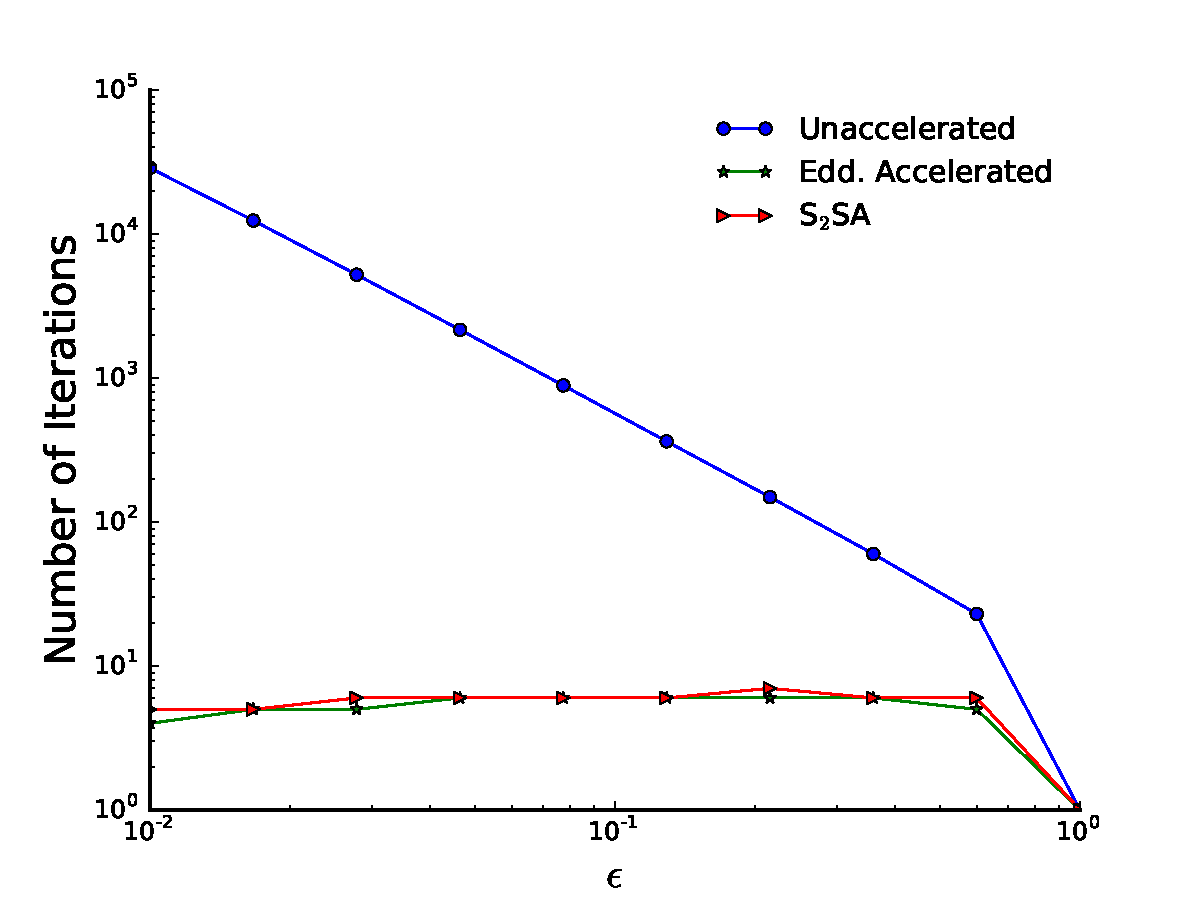
\includegraphics[width=.75\textwidth]{figs/diffLimit.pdf}
		\caption{The number of iterations for the VEF method to converge in the limit as $\epsilon \rightarrow 0$.}
		\label{fig:diffLim_iterations}
	\end{figure}
	\begin{figure} \centering
		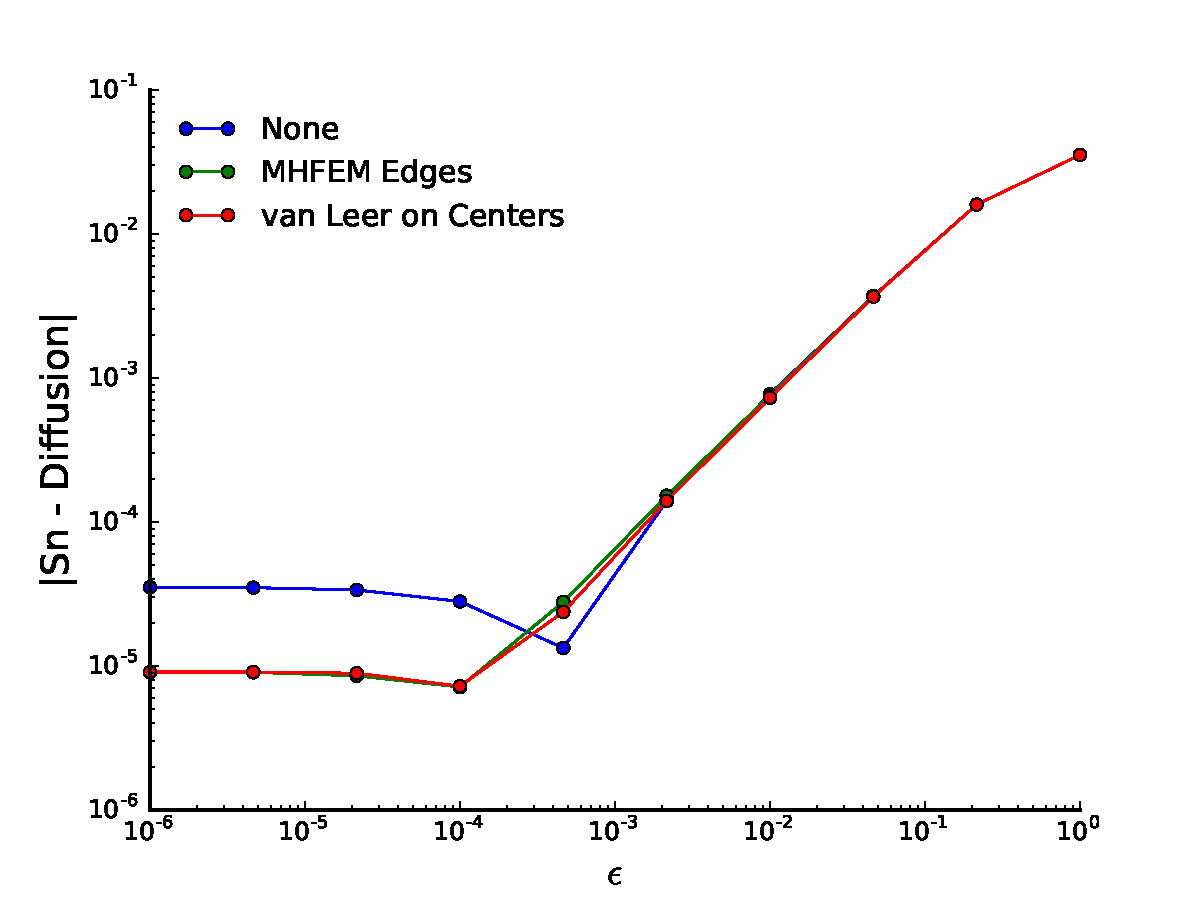
\includegraphics[width=.75\textwidth]{figs/diffError.pdf}
		\caption{A plot of the error between Diffusion Theory and the VEF solution as $\epsilon\rightarrow 0$. }
		\label{fig:diffLim_error}
	\end{figure}

\subsection{Solution Convergence}
The convergence between unaccelerated SI and the VEF method was compared as a function of cell width for a simple homogeneous slab and for a variant of Reed's problem. In both cases, the slab had a reflecting left boundary and vacuum right boundary. The homogeneous slab had a scattering ratio of 0.75. The cross sections and source for Reed's problem are provided in Table \ref{tab:reedXS}. Figure \ref{fig:reed} shows the L2 norm of the difference between unaccelerated and VEF accelerated S$_8$ for the two test problems. 

	\begin{table} \centering
		\begin{tabular}{|c|c|c|c|c|c|}
			\hline
			& Region 1 & Region 2 & Region 3 & Region 4 & Region 5 \\ 
			\hline 
			$q$ & 50 & 0 & 0 & 0 & 1 \\ 
			$\Sigma_t$ & 50 & 0.001 & 1 & 5 & 1 \\ 
			$\Sigma_a$ & 50 & 0 & 0.1 & 0 & 0.1 \\ 
			\hline 
			Domain & $0 \leq x < 2$ & $2 \leq x < 4$ & $4\leq x < 6$ &
				$6 \leq x < 7$ & $7 \leq x \leq 8$\\ 
			\hline 
		\end{tabular}
		\caption{The cross sections and source used for Reed's problem.}
		\label{tab:reedXS}
	\end{table}

	\begin{figure} \centering
		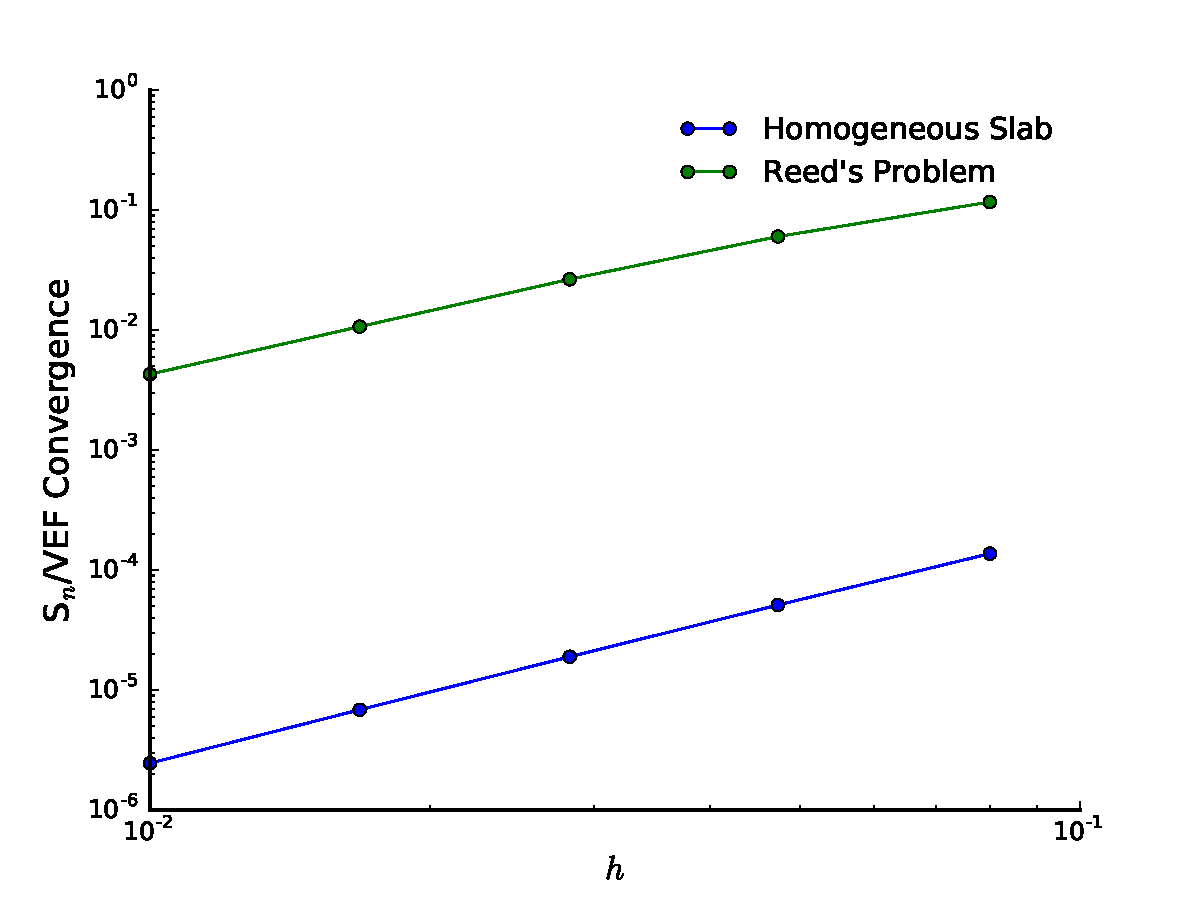
\includegraphics[width=.75\textwidth]{figs/convergence.pdf}
		\caption{The L2 norm of the difference between unaccelerated and VEF S$_8$ for a homogeneous slab and Reed's problem. }
		\label{fig:reed}
	\end{figure}

In both cases, the \SN and VEF solutions converge as the cell width is decreased. The convergence for Reed's problem is three orders of magnitudes worse than for the homogeneous slab case. This suggests that 

\subsection{Comparison to S$_2$SA}


%!TEX root = ./jctt.tex

\section{Computational Results}
\begin{figure}
\centering
\begin{subfigure}{.515\textwidth}
	\centering
	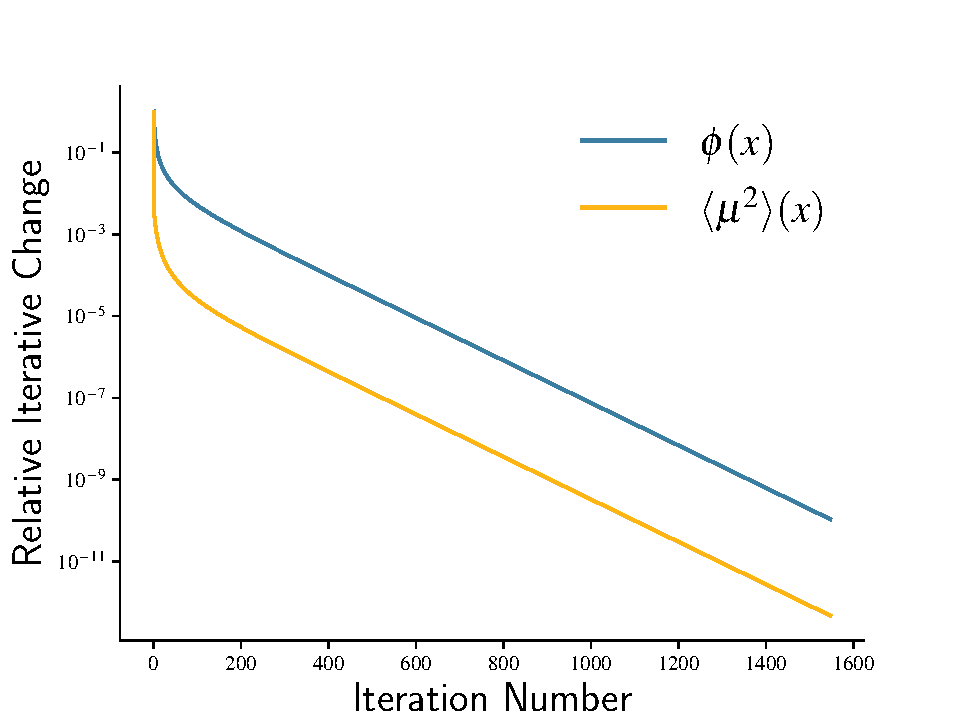
\includegraphics[width=\textwidth]{figs/si.pdf}
	\caption{}
	\label{fig:si}
\end{subfigure}
\hspace{-2em}
\begin{subfigure}{.515\textwidth}
	\centering
	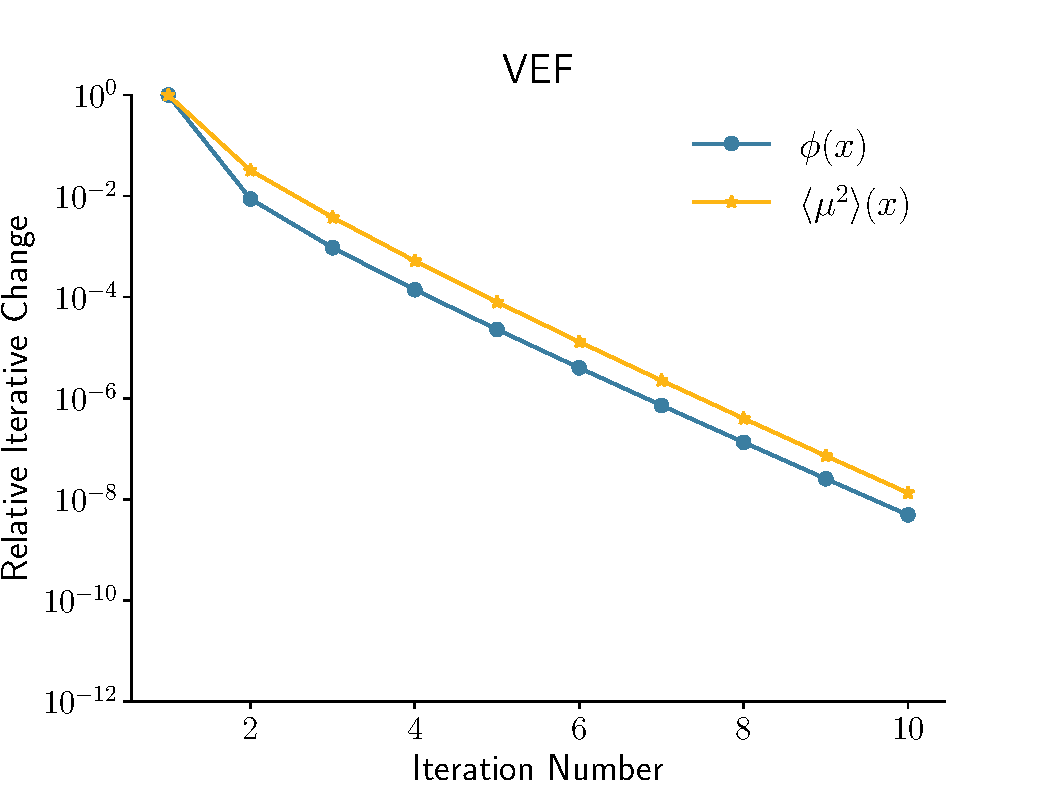
\includegraphics[width=\textwidth]{figs/vef.pdf} 
	\caption{}
	\label{fig:vef}
\end{subfigure}
\caption{The convergence rate for $\phi(x)$ and $\edd(x)$ for (a) unaccelerated and (b) VEF accelerated SI. }
\end{figure}

Figure \ref{fig:si} shows the convergence criterion
	\begin{equation}
		\frac{\| f\relll - f^\ell \|}{\| f\relll \|} 
	\end{equation}
as a function of unaccelerated iteration number for $f = \phi(x)$ and $f = \edd(x)$. The large drop in the convergence criterion between the first and second iterations supports the claim that the angular shape of the angular flux, and thus the Eddington factor, converges rapidly. When compared to Fig. \ref{fig:vef}, a plot of the convergence criterion versus number of iterations for the VEF method, it is clear that the VEF method transfers the fast rate of convergence of the Eddington factor to the scalar flux. 

	% \begin{figure}
	% 	\centering
	% 	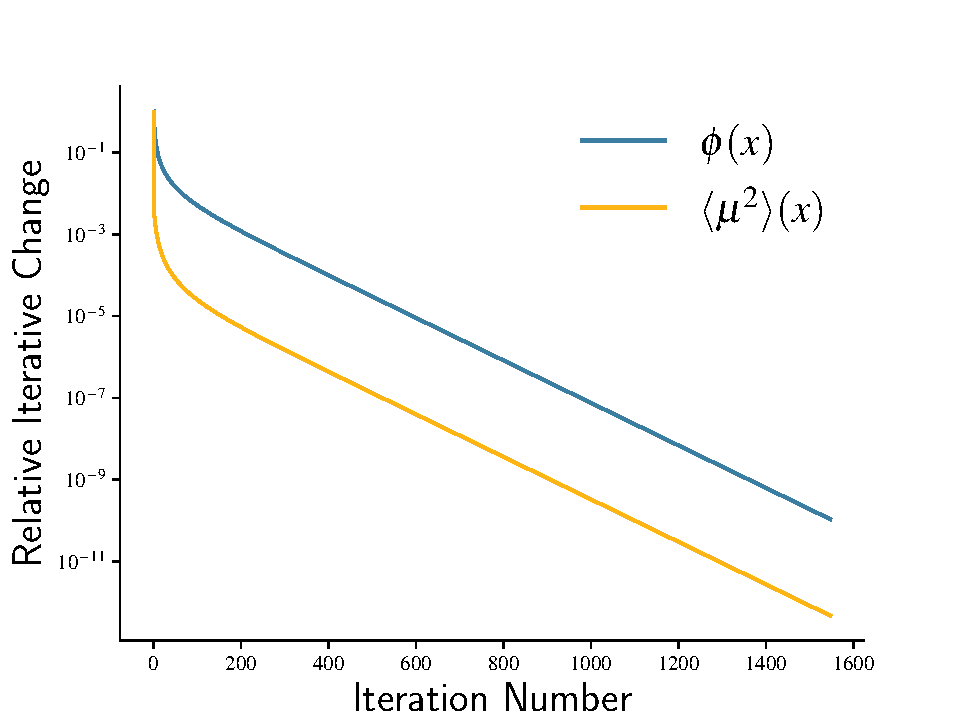
\includegraphics[width=.75\textwidth]{figs/si.pdf}
	% 	\caption{The convergence rate for $\phi(x)$ and $\edd(x)$ for unaccelerated S$_8$ Source Iteration. }
	% 	\label{fig:si}
	% \end{figure}

	% \begin{figure}
	% 	\centering
	% 	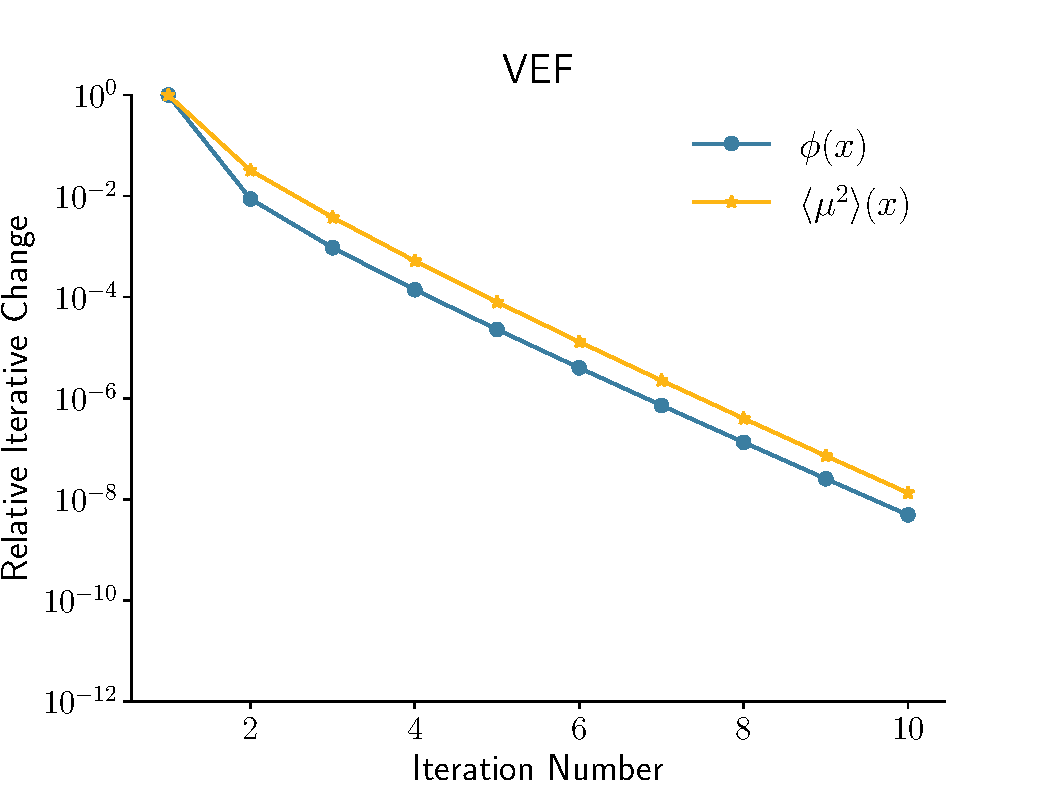
\includegraphics[width=.75\textwidth]{figs/vef.pdf} 
	% 	\caption{The convergence rate for $\phi(x)$ and $\edd(x)$ for VEF accelerated S$_8$. }
	% 	\label{fig:vef}
	% \end{figure}

To compare SI, VEF, and consistently differenced S$_2$SA, a test problem with a reflecting left boundary and a vacuum right boundary was used. This system was discretized into 50 spatial cells. $\sigma_t$ was set to \SI{1}{cm^{-1}} leading to an optical thickness per cell of 0.2. The convergence tolerance was set to \num{e-6}. Figure \ref{fig:si_vef_s2sa} shows the number of iterations required for convergence for SI, VEF, and S$_2$SA for varying ratios of $\sigma_s$ to $\sigma_t$. Aside from $\sigma_s/\sigma_t = 0$ where acceleration is not possible, the ratio of unaccelerated to VEF accelerated iterations ranged from 1.6 to 7. This suggests that acceleration is occurring and that the VEF method is not just doing twice the amount of work per iteration. In addition, the VEF method performed similarly to S$_2$SA. 

	\begin{figure}
		\centering
		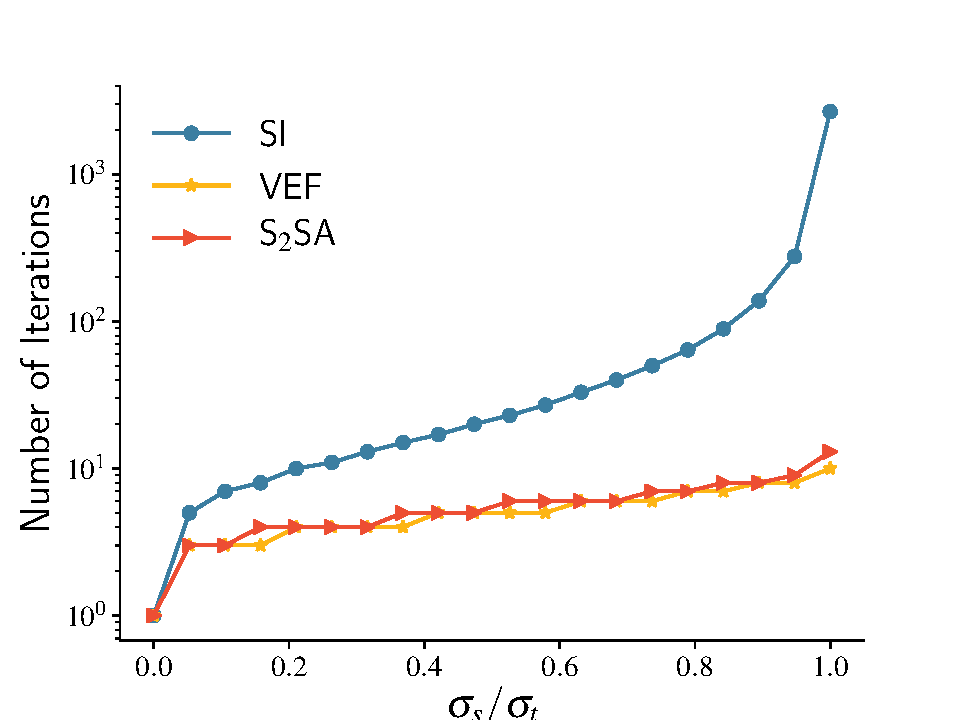
\includegraphics[width=.75\textwidth]{figs/si_vef_s2sa.pdf} 
		\caption{A comparison of the number of iterations required for Source Iteration, VEF acceleration, and S$_2$SA to converge for varying ratios of $\sigma_s$ to $\sigma_t$. } 
		\label{fig:si_vef_s2sa}
	\end{figure}

The Method of Manufactured Solutions (MMS) was used to compare the accuracy of the VEF method as the cell width was decreased. The L2 norm of the difference between the numerical and MMS solutions was compared at five logarithmically spaced cell widths between \SI{0.5}{mm} and \SI{0.01}{mm}. A line of best fit of the form 
	\begin{equation}
		E = C h^n
	\end{equation}
was used to find the order of accuracy, $n$, and the constant of proportionality, $C$, of the numerical error, $E$. These values are provided in Table \ref{tab:mms} for the permutations of the two reconstruction methods and two angular flux representation methods. All of the permutations are second order accurate and have similar overall accuracy. This suggests that slope reconstruction and angular flux representation do not affect numerical accuracy. It is also a testament to the robustness of the VEF method as the inconsistent, partially consistent, and fully consistent methods all performed similarly. 

	\begin{table} \centering
	\begin{tabular}{|c|c|c|c|c|}
	\hline
	\hline
	Reconstruction Method & $\psi$ Representation & Order & $C$ & $R^2$ \\ 
	\hline
		Flat & \num{1.979} & \num{1.18} & \num{9.9999e-01} \\
Linear & \num{1.988} & \num{0.786} & \num{9.9887e-01} \\

	\hline
	\hline
	\end{tabular}
	\caption{The order of accuracy, error, and $R^2$ values for the permutations of the two Eddington representation methods and two slope reconstruction methods. }
	\label{tab:mms}
	\end{table}
	\afterpage{\clearpage}

The convergence between unaccelerated SI and the VEF method was compared as a function of cell width for a simple homogeneous slab and for Reed's problem. In both cases, the left boundary was reflecting and the right boundary was vacuum. The homogeneous slab had a scattering ratio of 0.75. The cross sections and source for Reed's problem are provided in Table \ref{tab:reedXS}. The L2 norm of the difference between the SI solution and VEF solution is plotted for the four permutations of no reconstruction, van Leer slope limited reconstruction, constant angular flux representation, and linear angular flux representation in Figures \ref{fig:homo} and \ref{fig:reed} for the homogeneous slab problem and Reed's problem. 

	\begin{table} \centering
		\begin{tabular}{|c|c|c|c|c|c|}
			\hline
			& Region 1 & Region 2 & Region 3 & Region 4 & Region 5 \\ 
			\hline 
			$q$ & 50 & 0 & 0 & 0 & 1 \\ 
			$\Sigma_t$ & 50 & 0.001 & 1 & 5 & 1 \\ 
			$\Sigma_a$ & 50 & 0 & 0.1 & 0 & 0.1 \\ 
			\hline 
			Domain & $0 \leq x < 2$ & $2 \leq x < 4$ & $4\leq x < 6$ &
				$6 \leq x < 7$ & $7 \leq x \leq 8$\\ 
			\hline 
		\end{tabular}
		\caption{The cross sections and source used for Reed's problem.}
		\label{tab:reedXS}
	\end{table}

	\begin{figure}
		\centering
		\begin{subfigure}{.5\textwidth}
			\centering
			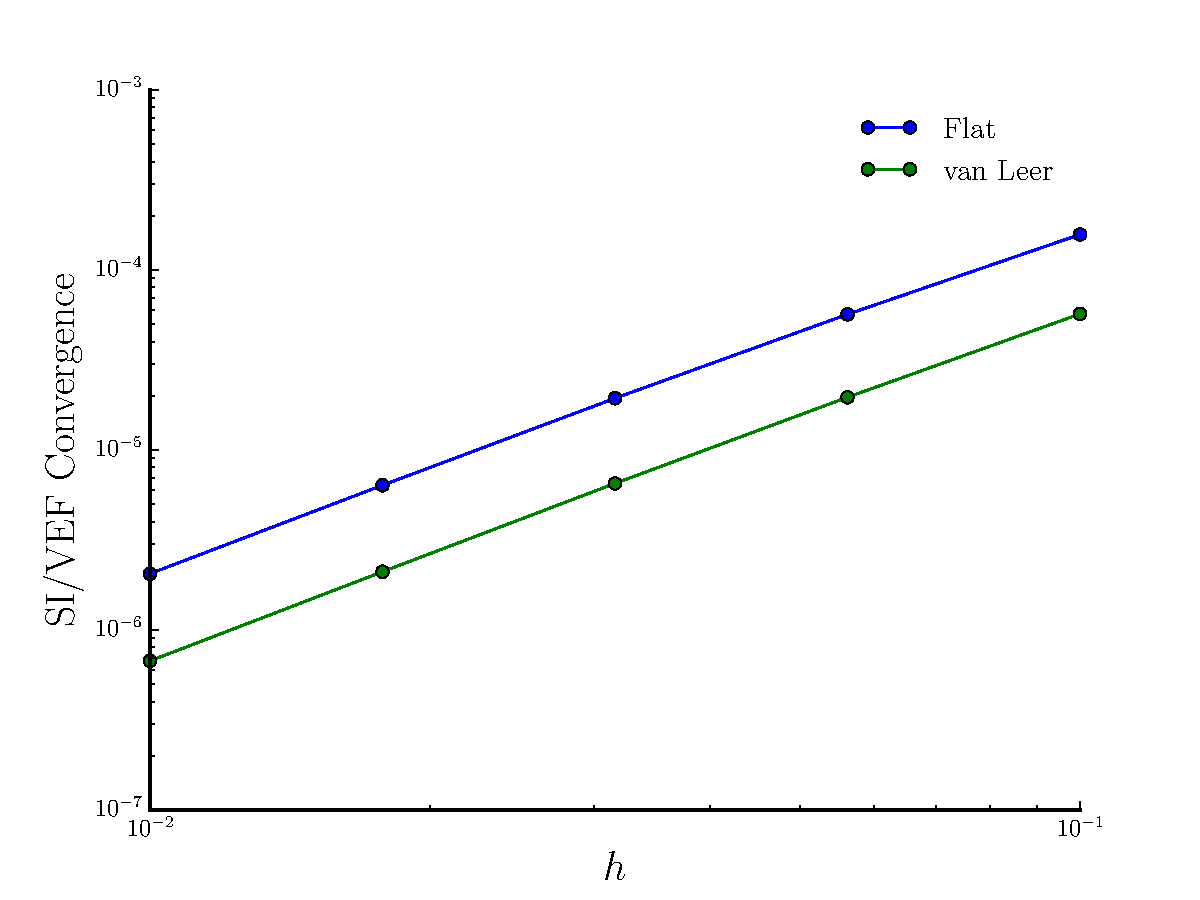
\includegraphics[width=\textwidth]{figs/solconv_homo.pdf}
			\caption{}
			\label{fig:homo}
		\end{subfigure}
		\hspace{-2em}
		\begin{subfigure}{.5\textwidth}
			\centering
			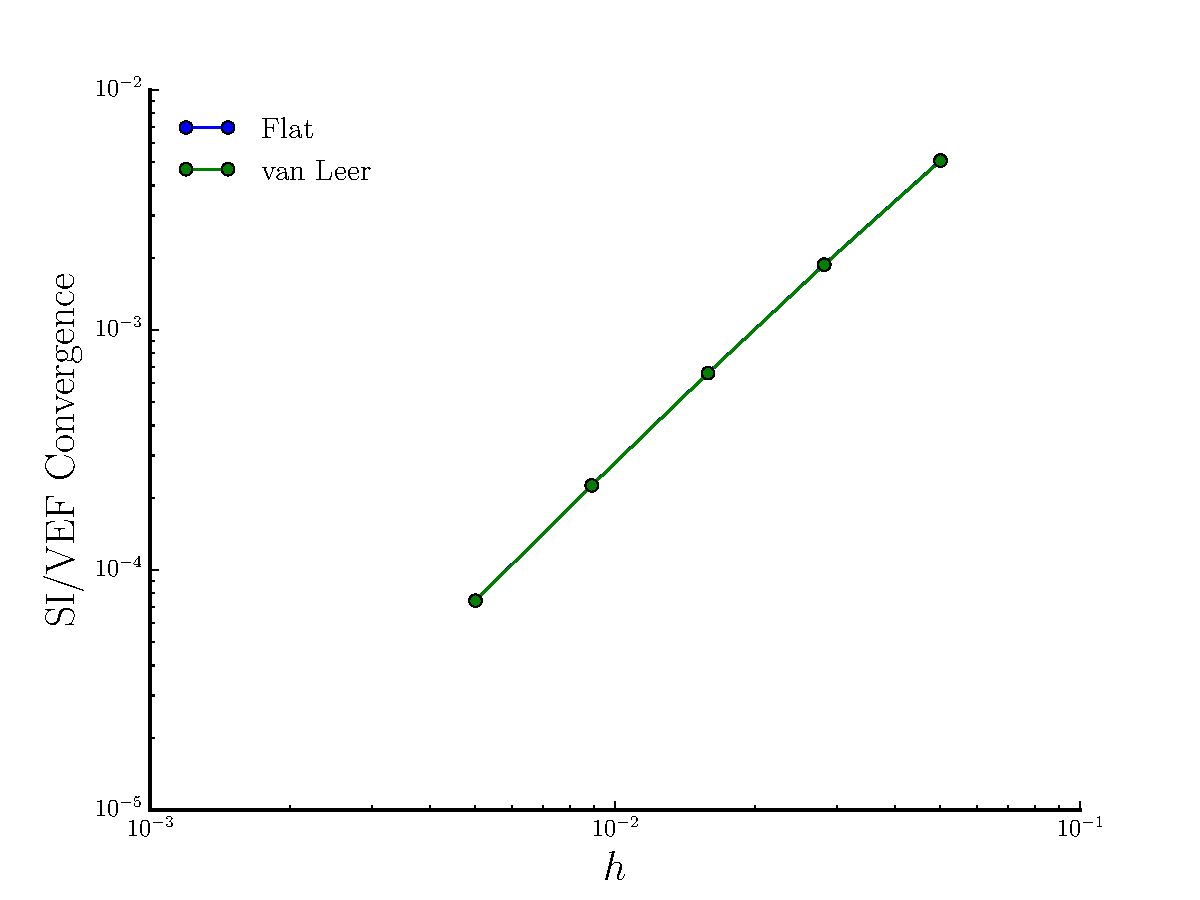
\includegraphics[width=\textwidth]{figs/solconv_reed.pdf}
			\caption{}
			\label{fig:reed}
		\end{subfigure}
		\caption{The L2 norm of the difference between SI and the four permutations of the VEF method as the cell spacing is decreased for (a) the homogeneous slab problem and (b) Reed's problem. }
	\end{figure}

In the homogeneous problem, VEF with van Leer limited slope reconstruction was five times more convergent than VEF without reconstruction. Use of the linear angular flux representation decreased the van Leer reconstruction convergence by 30\%. In Reed's problem, all four methods performed similarly. This suggests that the effects of the linear representation of the angular flux is problem dependent. However, slope reconstruction greatly increased solution convergence. 

Lastly, slope reconstruction and angular flux representation were tested in the diffusion limit. The cross sections and source were scaled according to: 
	\begin{subequations} \label{res:scaling}
		\begin{equation} 
			\sigma_t(x) \rightarrow \sigma_t(x)/\epsilon \,, 
		\end{equation}
		\begin{equation}
			\sigma_s(x) \rightarrow \epsilon \sigma_s(x) \,,
		\end{equation}
		\begin{equation}
			Q(x) \rightarrow \epsilon Q(x) \,. 
		\end{equation}
	\end{subequations}
As $\epsilon \rightarrow 0$, the system becomes diffusive. The number of iterations for convergence within a tolerance of \num{e-10} as $\epsilon \rightarrow 0$ is plotted in Fig. \ref{fig:dl_it}. The error between the VEF solution and the exact diffusion solution is provided in Fig. \ref{fig:dl_err}. This supports the claim that the VEF method is robust as all four permutations survived the diffusion limit. 
	
	\begin{figure}
		\centering
		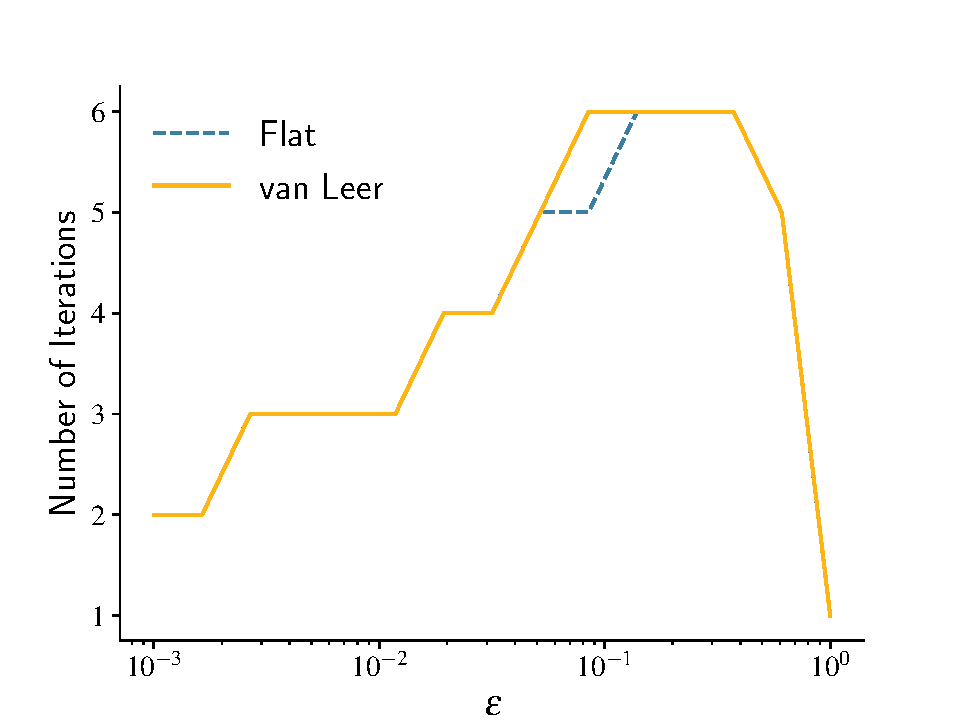
\includegraphics[width=.75\textwidth]{figs/dl_it.pdf}
		\caption{The number of iterations required for convergence for the permutations of slope reconstruction and angular flux representation in the diffusion limit. }
		\label{fig:dl_it}
	\end{figure}
	\begin{figure}
		\centering
		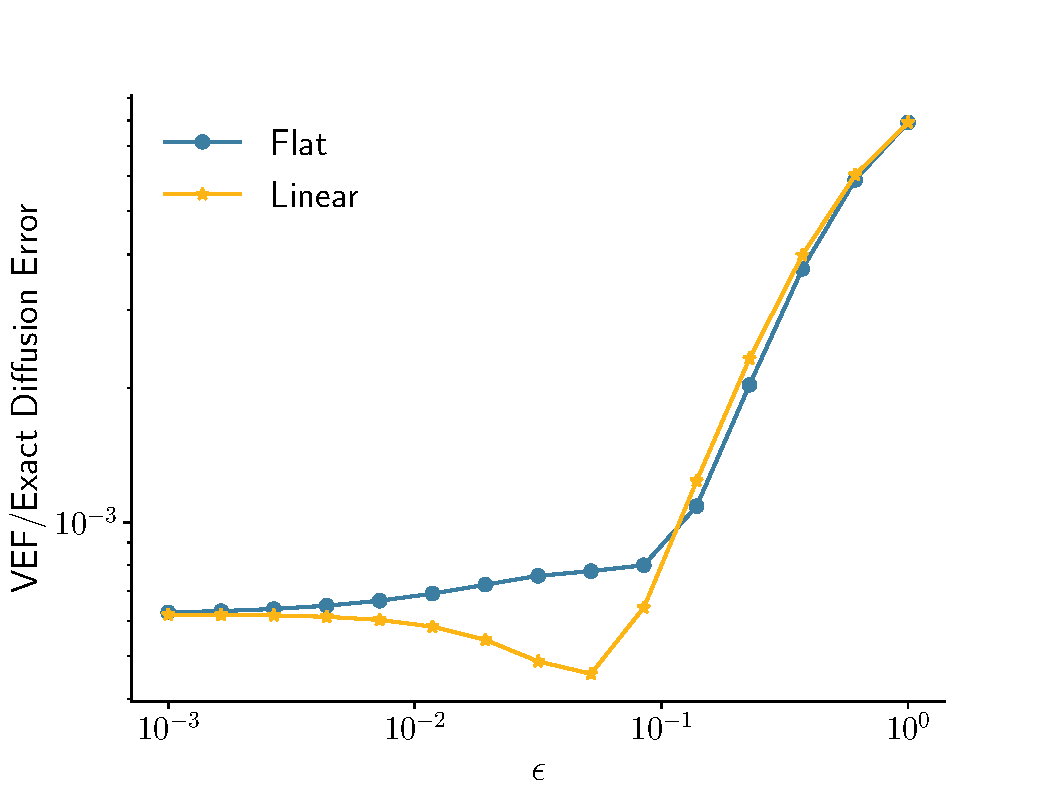
\includegraphics[width=.75\textwidth]{figs/dl_err.pdf}
		\caption{The error between the VEF methods and the exact diffusion solution as $\epsilon \rightarrow 0$. }
		\label{fig:dl_err}
	\end{figure}

%!TEX root = ./jctt.tex

\section{Conclusions and Future Work}
We have presented the VEF method for one-group neutron transport in slab geometry and the pairing of LLDG for the \SN transport step and MFEM for the drift diffusion acceleration step. We have numerically demonstrated that the LLDG/MFEM VEF method accelerates Source Iteration by transferring the rapid convergence of the angular shape of the angular flux to the scalar flux. The VEF method performed similarly to consistently differenced S$_2$SA. 

Methods for increased consistency between LLDG and MFEM were also presented. This included a cell centered slope reconstruction method that will be needed for radiative transfer calculations. It was shown that that the inconsistent, partially consistent, and fully consistent methods were second-order accurate as expected from the orders of accuracy of LLDG and MFEM in isolation and that all of the VEF methods were robust in the diffusion limit. In addition, while this nonlinear scheme produces two solutions, one from \SN and one from drift diffusion, the solutions were shown to converge as the mesh was refined for both homogeneous and inhomogeneous systems. 

% add rational polynomial conclusions: expected to be important in rad transfer 
% mfem is conservative and can be paired to multiphysics 
% take out consistency talk 

Future work includes extending the VEF method presented in this paper to the radiative transfer equations and verifying the VEF method in 2 and 3 dimensional systems. 

\bibliographystyle{unsrt}
\bibliography{references}
\end{document}